\documentclass[11pt,a4paper]{article}
\usepackage[utf8]{inputenc}
\usepackage[T1]{fontenc}
\usepackage{tgpagella}
\usepackage[spanish]{babel}
\usepackage{geometry}
\usepackage{booktabs}
\usepackage{xcolor}
\usepackage{titlesec}
\usepackage{fancyhdr}
\usepackage[parfill]{parskip}
\usepackage[expansion=false]{microtype}
\usepackage{hyperref}
\usepackage{setspace}
\usepackage{needspace}
\usepackage{graphicx}
\widowpenalty=10000
\clubpenalty=10000
\displaywidowpenalty=10000

\geometry{top=3.0cm,bottom=3.0cm,left=3.5cm,right=3.5cm}
\setlength{\parskip}{0.65em}
\setlength{\parindent}{0em}

\definecolor{azulai}{RGB}{30,80,140}
\definecolor{doradoai}{RGB}{140,90,0}
\definecolor{grisai}{RGB}{70,70,70}

\titleformat{\section}{\Large\bfseries\color{azulai}}{}{0em}{}[{\color{azulai}\titlerule[0.5pt]}]
\titlespacing*{\section}{0pt}{1.8em}{0.8em}
\titleformat{\subsection}{\large\bfseries\color{doradoai}}{}{0em}{}
\titlespacing*{\subsection}{0pt}{1.4em}{0.5em}
\titleformat{\subsubsection}{\normalsize\bfseries\color{grisai}}{}{0em}{}
\titlespacing*{\subsubsection}{0pt}{1.0em}{0.3em}

\pagestyle{fancy}\fancyhf{}
\rhead{\textcolor{grisai}{\small Raquel Pain — Arquitectura Interna}}
\lhead{\textcolor{grisai}{\small Sol · Ascendente · Nodos}}
\cfoot{\textcolor{grisai}{\small\thepage}}
\renewcommand{\headrulewidth}{0.3pt}

\hypersetup{colorlinks=true,linkcolor=azulai,urlcolor=azulai}
\setstretch{1.45}
\tolerance=1500
\emergencystretch=4em

\begin{document}

% ── Portada ──────────────────────────────────────────────────────────────────
\begin{titlepage}
  \centering
  \vspace*{1.5cm}
  {\Huge\bfseries\color{azulai} Sol · Ascendente · Nodos}\\[0.5cm]
  {\large\color{grisai} Arquitectura Interna}\\[0.3cm]
  {\small\itshape\color{grisai} Dirección vital, punto de entrada y eje de desarrollo}\\[2cm]
  {\huge\color{doradoai} Raquel Pain}\\[1.5cm]
  {\Large 07/05/1985 \quad 18:20}\\[0.3cm]
  {\Large Pamplona, España}\\[0.3cm]
  {\normalsize Lat: 42.8157° \quad Lon: -1.6522° \quad UTC+02:00}\\[0.3cm]
  {\normalsize Ascendente: Libra 14°36' \quad
    MC: Cáncer 17°21'}\\[2cm]
  \begin{tabular}{lll}
    \textbf{Sol:} & Tauro & Casa 8 \\
    \textbf{Ascendente:} & Libra & Punto de entrada principal: Venus \\
    \textbf{Nodo Norte:} & Tauro & Casa 8 \\
    \textbf{Nodo Sur:}   & Escorpio & Casa 2 \\
  \end{tabular}\\[2cm]
  \vfill
  {\small Generado el 20/05/2026}
\end{titlepage}

\tableofcontents
\newpage

% ── Datos de referencia ───────────────────────────────────────────────────────
\section{Datos de referencia}

\begin{center}
\begin{tabular}{llll}
  \toprule
  \textbf{Punto} & \textbf{Signo} & \textbf{Casa} & \textbf{Posición} \\
  \midrule
  Sol           & Tauro & 8 & 17°02' \\
  Ascendente    & Libra & --- & 14°36' \\
  Medio Cielo   & Cáncer & --- & 17°21' \\
  Nodo Norte    & Tauro & 8 & 18°11' \\
  Nodo Sur      & Escorpio & 2 & 18°11' \\
  \bottomrule
\end{tabular}
\end{center}

\vspace{0.5cm}
\textbf{Regente del Ascendente (Libra):} 
Venus —
Aries, 
Casa 6

\vspace{0.5cm}
\textbf{Aspectos entre Sol, Ascendente y Nodos:}

\begin{center}
\begin{tabular}{lllll}
  \toprule
  \textbf{Planeta 1} & \textbf{Asp.} & \textbf{Planeta 2} & \textbf{Tipo} & \textbf{Orbe} \\
  \midrule
  Sol & = & Nodo Norte & Conjunción & 1.1° \\
  Sol & ☍ & Nodo Sur & Oposición & 1.1° \\
  Sol & ⚻ & Ascendente & Quincuncio & 2.4° \\
  Nodo Norte & ⚻ & Ascendente & Quincuncio & 3.6° \\
  \bottomrule
\end{tabular}
\end{center}

\needspace{3\baselineskip}
\subsection*{Grados sensibles}



\vspace{0.7cm}

\begin{center}
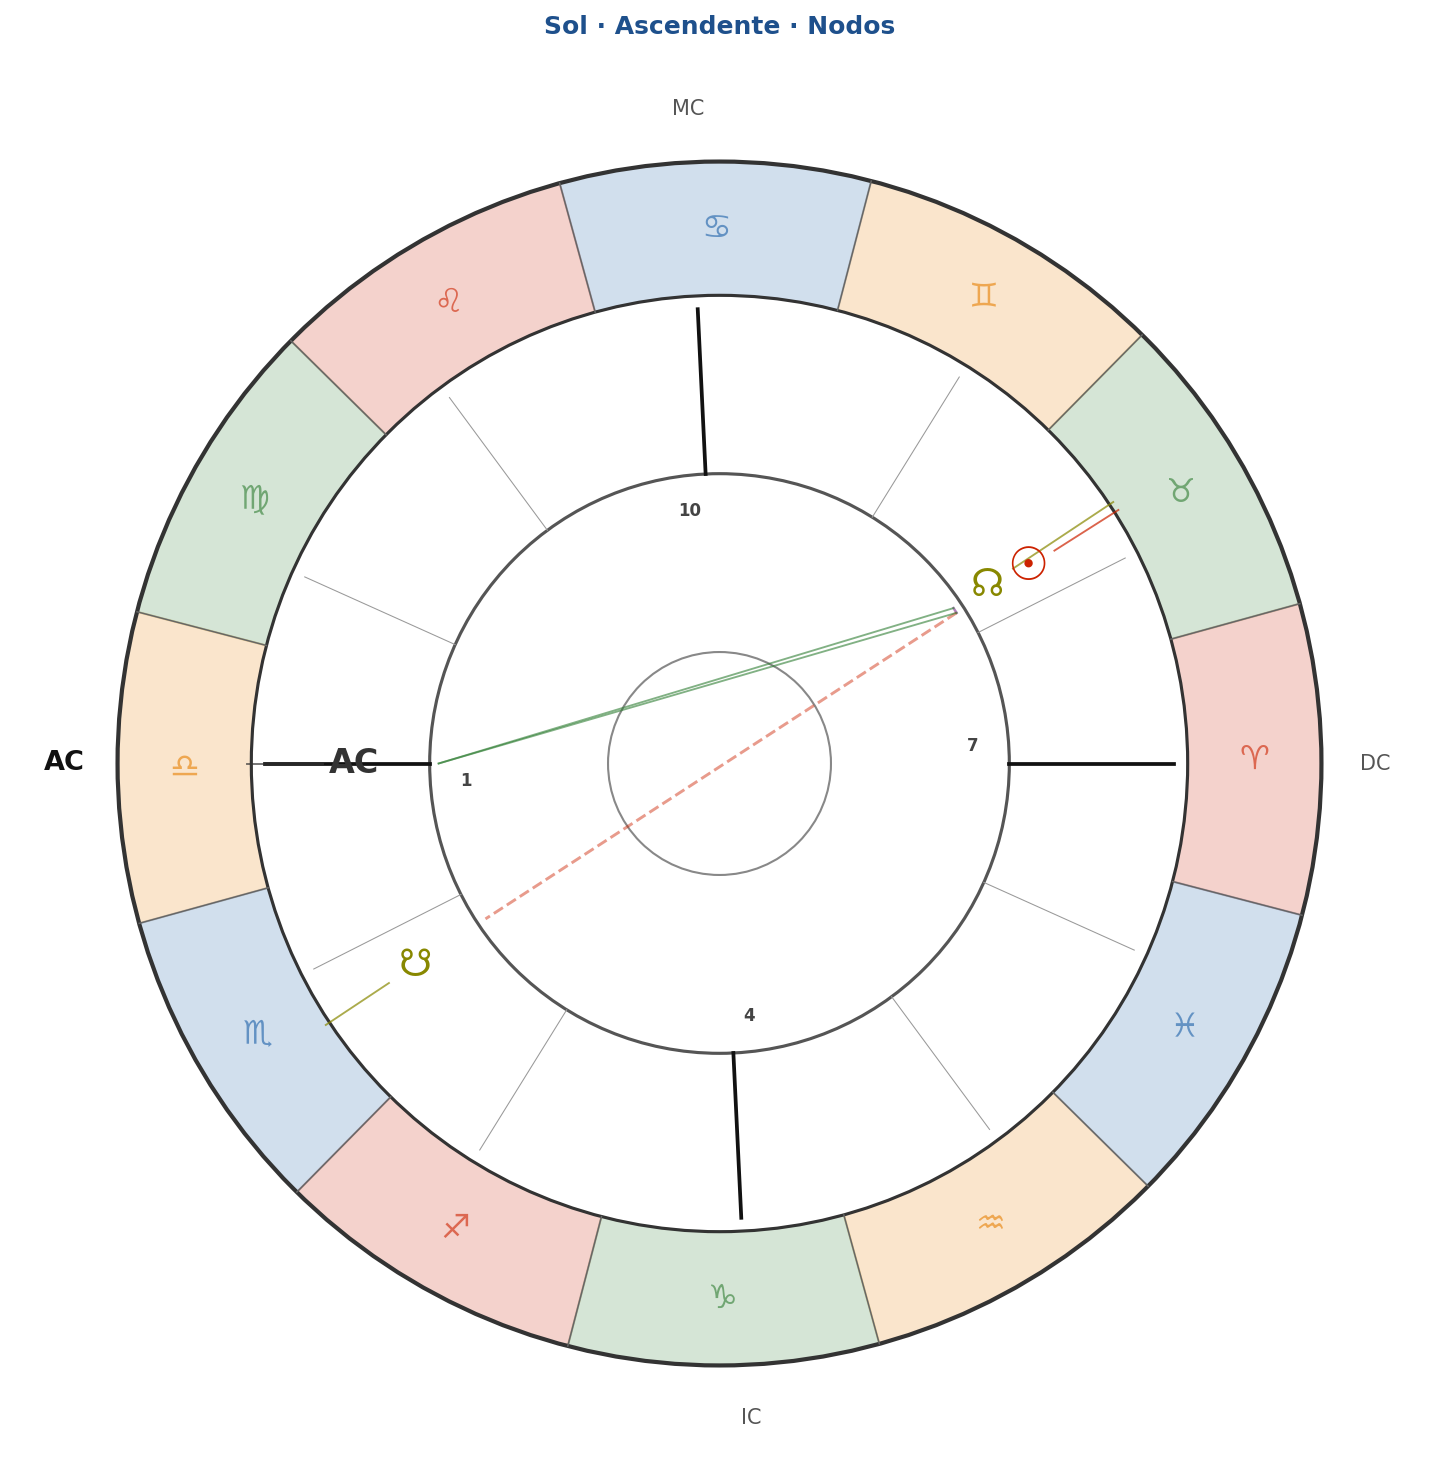
\includegraphics[width=0.72\textwidth]{Raquel_Pain_Sol_ASC_Nodos_rueda.png}
\end{center}


\vspace{0.3cm}
\Needspace{5\baselineskip}

% ── Interpretación ────────────────────────────────────────────────────────────
\section{Interpretación — Arquitectura Interna}

\begin{center}
{\small\itshape
No se trata de definir quién eres. Se trata de observar cómo se organiza tu dirección,
cómo atraviesas la vida y qué tensión influye en tu forma de avanzar.
}
\end{center}

\vspace{0.5cm}
\Needspace{5\baselineskip}


% ── 1. Dirección general ──────────────────────────────────────────────────────
\needspace{3\baselineskip}
\subsection{1. Dirección general}

El Sol está en Tauro, Casa 8. El Ascendente está en Libra. El Nodo Norte está en Tauro, Casa 8, y el Nodo Sur en Escorpio, Casa 2.

El Sol en Tauro y el Ascendente en Libra pertenecen a elementos con lógicas diferentes. Esto puede hacer que vivas las cosas de una forma, mientras otra parte de ti necesita orientarse desde un ritmo completamente diferente. Además, el Sol hace quincuncio con el Ascendente (orbe 2.44°), por lo que esta relación tiene un peso especial en la carta.

El Sol y el Nodo Norte están en Tauro. Esto une tu dirección principal con una zona importante de crecimiento. Puede haber una sensación más clara de hacia dónde avanzar, aunque eso no significa que el trabajo ya esté hecho.

El Nodo Norte hace quincuncio con el Ascendente (orbe 3.59°). Esto indica que la dirección de crecimiento también toca directamente tu manera de entrar en la vida y posicionarte.

\vspace{0.5cm}
\Needspace{5\baselineskip}


% ── 2. Sol ────────────────────────────────────────────────────────────────────
\needspace{3\baselineskip}
\subsection{2. El Sol — Dirección principal}

\needspace{3\baselineskip}
\subsubsection*{Sol en Tauro · Casa 8}

Tu dirección se activa cuando puedes construir algo poco a poco. Necesitas estabilidad, continuidad y sentir que el esfuerzo tiene una forma concreta. Las prisas suelen bloquearte más de lo que ayudan.

Funcionas mejor cuando tienes tiempo para consolidar lo que haces, entender tus ritmos y avanzar de manera gradual. Cuando todo cambia demasiado rápido o el entorno exige respuestas inmediatas, puedes cerrarte, resistirte o quedarte parado más tiempo del que desearías.

Te afecta mucho perder aquello que habías construido, sentir que no hay suelo firme o vivir cambios constantes sin preparación. La dirección aparece cuando puedes echar raíces en lo que haces.

Tu dirección aparece cuando puedes atravesar procesos de cambio reales y profundos. Necesitas sentir que lo que haces transforma algo importante.

Las dinámicas superficiales o demasiado controladas suelen dejarte vacío rápidamente. También te afecta mucho acumular emociones, tensión o situaciones no resueltas durante demasiado tiempo.

Cuando puedes entrar en profundidad y transformar lo que ya no sirve, recuperas fuerza y claridad.

El Sol y el Nodo Norte apuntan hacia la misma dirección. Existe una sensación más natural de avanzar hacia aquello que necesitas desarrollar y muchas veces ciertas decisiones importantes se sienten coherentes internamente incluso cuando requieren esfuerzo o implican atravesar incomodidad. La dirección suele percibirse con más claridad que en otras configuraciones y puede existir sensación de que algunas experiencias importantes encajan profundamente con lo que necesitas construir. El reto está en no confundir facilidad con trabajo ya realizado. A veces el crecimiento parece tan natural que cuesta ver cuándo sigues funcionando desde patrones antiguos o demasiado conocidos.

El Sol se opone al Nodo Sur y apunta hacia el Nodo Norte. La dirección de crecimiento suele sentirse mucho más visible y alineada con tu impulso vital y con aquello que necesitas construir hacia adelante. Aun así, el Nodo Sur continúa funcionando como un lugar de regreso automático en momentos de cansancio, miedo o exceso de presión. Lo antiguo sigue teniendo fuerza aunque ya no sea el lugar principal de desarrollo. El reto está en no idealizar únicamente la dirección de crecimiento olvidando que también necesitas comprender y ordenar aquello que dejas atrás.

El Sol y el Ascendente necesitan reajustes continuos entre lo que haces espontáneamente y la dirección más profunda de tu vida. Puede existir sensación de tener que modificar constantemente la manera de actuar, relacionarte o posicionarte para sentir más coherencia interna. A veces lo que surge automáticamente no termina de encajar del todo con lo que realmente necesitas construir o desarrollar a largo plazo. El reto está en aceptar que aquí el equilibrio rara vez aparece de una vez para siempre y suele construirse poco a poco mediante ajustes repetidos.


\vspace{0.5cm}
\Needspace{5\baselineskip}


% ── 3. Ascendente ─────────────────────────────────────────────────────────────
\needspace{3\baselineskip}
\subsection{3. El Ascendente — Forma de relacionarte con la vida}

\needspace{3\baselineskip}
\subsubsection*{Libra · Regente: Venus}

Lo que vives suele tomar forma a través de las relaciones y del contacto con otras personas.Necesitas contraste, intercambio y cierta referencia externa para aclarar cómo te posicionas frente a lo que ocurre.

Cuando pasas demasiado tiempo sin diálogo, sin referencias o en relaciones tensas y desequilibradas, es fácil quedarte en suspensión y no saber bien hacia dónde moverte.

Te ayuda poder pensar junto a otras personas y sentir que hay espacio para el acuerdo, el ajuste y la negociación.

El regente del Ascendente es Venus, situado en Aries, Casa 6. Venus pertenece a un elemento compatible con el Ascendente. Esto puede facilitar que tu primera reacción y la forma en que después elaboras lo que ocurre se apoyen con cierta fluidez. La Casa 6 muestra un territorio importante desde el que organizas tu forma de entrar en la vida.

El Sol y el Ascendente necesitan reajustes continuos entre lo que haces espontáneamente y la dirección más profunda de tu vida. Puede existir sensación de tener que modificar constantemente la manera de actuar, relacionarte o posicionarte para sentir más coherencia interna. A veces lo que surge automáticamente no termina de encajar del todo con lo que realmente necesitas construir o desarrollar a largo plazo. El reto está en aceptar que aquí el equilibrio rara vez aparece de una vez para siempre y suele construirse poco a poco mediante ajustes repetidos.

La dirección de crecimiento requiere ajustes constantes en tu forma habitual de reaccionar y posicionarte frente a la vida. Muchas veces crecer implica modificar patrones muy automáticos de comportamiento o maneras antiguas de responder a lo que ocurre. Puede existir sensación de incomodidad porque aquello que antes funcionaba ya no termina de encajar completamente con la dirección actual de desarrollo. El crecimiento aquí rara vez se siente completamente estable y suele aparecer a través de pequeños reajustes repetidos. El reto está en aceptar que esa incomodidad forma parte natural del proceso y no significa necesariamente que estés yendo en la dirección equivocada.

\vspace{0.5cm}
\Needspace{5\baselineskip}


% ── 4. Nodos ──────────────────────────────────────────────────────────────────
\needspace{3\baselineskip}
\subsection{4. Nodo Norte y Nodo Sur — Dirección de crecimiento}

\needspace{3\baselineskip}
\subsubsection*{Nodo Norte en Tauro · Casa 8 \\
Nodo Sur en Escorpio · Casa 2}

Tu dirección pide construir algo estable, sencillo y sostenible en el tiempo. Aprender a confiar más en lo concreto, desarrollar recursos propios y permitirte ir más despacio sin sentir que pierdes profundidad. Lo conocido suele llevarte hacia la intensidad emocional, las crisis o los procesos de transformación constante. Puede existir una sensación de que solo aquello que remueve mucho es verdaderamente importante o real. El reto está en descubrir que la calma, la estabilidad y lo cotidiano también pueden contener muchísima profundidad. Crecer hacia este Nodo Norte implica dejar de necesitar continuamente situaciones límite para sentir que algo tiene valor.

Tu dirección pide entrar más profundamente en los procesos de cambio y transformación. Aprender a soltar lo que ya terminó y atravesar etapas donde no todo puede permanecer bajo control. El crecimiento aparece cuando puedes dejar atrás viejas seguridades y permitir que algunas partes de tu vida cambien de verdad en lugar de sostenerlas únicamente por miedo a perder estabilidad. El reto suele estar en no quedarte únicamente en lo conocido o en lo seguro por miedo a atravesar incertidumbre o intensidad emocional.

Sueles vivir lo que te pasa con mucha intensidad y profundidad, como si las experiencias necesitaran transformarte de alguna manera. Hay facilidad para entrar en lo complejo, sostener crisis o percibir lo que otras personas no ven, pero también tendencia a permanecer en tensión emocional constante. Puede aparecer sensación de que solo aquello que remueve mucho, duele o tiene gran intensidad emocional es verdaderamente importante o real. El problema surge cuando necesitas conflicto, profundidad extrema o intensidad permanente para sentir conexión con la vida.

Tiendes a buscar seguridad en lo conocido, en lo estable y en aquello que puedes controlar, conservar o sostener de forma concreta. Hay facilidad para construir recursos y mantener continuidad en el tiempo, pero también dificultad para entrar en cambios profundos cuando implican incertidumbre o pérdida de referencias conocidas. Muchas veces aparece necesidad de aferrarte a estructuras, vínculos o situaciones que ofrecen estabilidad aunque ya no estén verdaderamente vivos. El problema surge cuando mantener seguridad se vuelve más importante que reconocer que algo necesita transformarse.

El Sol y el Nodo Norte apuntan hacia la misma dirección. Existe una sensación más natural de avanzar hacia aquello que necesitas desarrollar y muchas veces ciertas decisiones importantes se sienten coherentes internamente incluso cuando requieren esfuerzo o implican atravesar incomodidad. La dirección suele percibirse con más claridad que en otras configuraciones y puede existir sensación de que algunas experiencias importantes encajan profundamente con lo que necesitas construir. El reto está en no confundir facilidad con trabajo ya realizado. A veces el crecimiento parece tan natural que cuesta ver cuándo sigues funcionando desde patrones antiguos o demasiado conocidos.

El Sol se opone al Nodo Sur y apunta hacia el Nodo Norte. La dirección de crecimiento suele sentirse mucho más visible y alineada con tu impulso vital y con aquello que necesitas construir hacia adelante. Aun así, el Nodo Sur continúa funcionando como un lugar de regreso automático en momentos de cansancio, miedo o exceso de presión. Lo antiguo sigue teniendo fuerza aunque ya no sea el lugar principal de desarrollo. El reto está en no idealizar únicamente la dirección de crecimiento olvidando que también necesitas comprender y ordenar aquello que dejas atrás.

La dirección de crecimiento requiere ajustes constantes en tu forma habitual de reaccionar y posicionarte frente a la vida. Muchas veces crecer implica modificar patrones muy automáticos de comportamiento o maneras antiguas de responder a lo que ocurre. Puede existir sensación de incomodidad porque aquello que antes funcionaba ya no termina de encajar completamente con la dirección actual de desarrollo. El crecimiento aquí rara vez se siente completamente estable y suele aparecer a través de pequeños reajustes repetidos. El reto está en aceptar que esa incomodidad forma parte natural del proceso y no significa necesariamente que estés yendo en la dirección equivocada.

\vspace{0.5cm}
\Needspace{5\baselineskip}


% ── 5. Integración ────────────────────────────────────────────────────────────
\needspace{3\baselineskip}
\subsection{5. Integración — Cómo se relacionan las distintas partes}

El Ascendente en Libra y el Sol en Tauro pertenecen a elementos con lógicas diferentes. Esto puede hacer que una parte de ti quiera vivir las cosas de una forma, mientras otra necesita avanzar desde un ritmo completamente diferente.Cuando no hay espacio para traducir esas dos formas internas, puedes sentir que reaccionas por un lado y deseas orientarte por otro. El trabajo está en no forzarte a elegir una sola parte, sino en aprender a darles un lugar más coherente.

Además, el Sol hace quincuncio con el Ascendente (orbe 2.44°). Esto refuerza la importancia de observar cómo se relacionan tu manera de entrar en la vida y tu dirección principal.

El Sol y el Nodo Norte están en Tauro. Esto une tu dirección principal con una zona importante de crecimiento. Puede darte una sensación más clara de hacia dónde avanzar, pero no significa que ese camino ya esté integrado. El reto está en no dar por hecho que lo natural ya está plenamente desarrollado.

El Ascendente en Libra y el Nodo Norte en Tauro pertenecen a elementos con lógicas diferentes. Esto puede hacer que crecer te pida actuar de una manera que no siempre coincide con tu primera reacción. El trabajo está en aprender a no obedecer siempre al primer impulso y dejar espacio a una dirección más nueva.

Además, el Nodo Norte hace quincuncio con el Ascendente (orbe 3.59°). Esto hace que la dirección de crecimiento toque directamente tu forma de posicionarte en la vida.

\vspace{0.5cm}
\Needspace{5\baselineskip}


% ── 6. Orientación práctica ───────────────────────────────────────────────────
\needspace{3\baselineskip}
\subsection{6. Orientación práctica}

\needspace{3\baselineskip}
\subsubsection*{Desde dónde empezar}
Desde el Ascendente en Libra: poner en palabras lo que está ocurriendo. Hablar sobre ello, escribirlo o compartirlo con alguien puede ayudarte a comprender mejor lo que estás viviendo. El Sol hace quincuncio con el Ascendente (orbe 2.44°), así que conviene observar especialmente cómo se relacionan tu primera reacción y tu dirección principal.

\needspace{3\baselineskip}
\subsubsection*{Qué conviene sostener}
El Sol en Tauro, Casa 8, necesita construir algo concreto y sostenible. Te ayuda avanzar paso a paso y ver que lo que haces va tomando forma.

\needspace{3\baselineskip}
\subsubsection*{Qué conviene observar}
Evita funcionar únicamente desde el Nodo Sur en Escorpio, Casa 2. Ese lugar puede resultarte conocido y eficaz, pero no debería convertirse en la única respuesta disponible. La señal de alerta aparece cuando resuelves siempre desde lo que ya sabes hacer, sin preguntarte si esa respuesta sigue siendo adecuada.

El Nodo Norte en Tauro, Casa 8, pide desarrollar una forma nueva de orientarte, aunque al principio resulte menos automática.

Hay una tensión importante entre Sol y Nodo Sur por oposición (orbe 1.15°). No hace falta resolverla de golpe. Lo importante es aprender a reconocer cuándo esa tensión te bloquea y cuándo puede convertirse en una forma más consciente de elegir.

El Nodo Norte hace quincuncio con el Ascendente (orbe 3.59°). Esto hace que tu dirección de crecimiento esté muy ligada a la manera en que te posicionas ante la vida.

\vspace{1cm}

\begin{center}
{\small\itshape\color{grisai}
La astrología se utiliza aquí como una herramienta de observación y orientación.
No define quién eres ni determina lo que va a ocurrir.
}
\end{center}

\end{document}
